\documentclass[a4paper,11pt]{article}
\usepackage{amsmath,amsthm,amssymb}
\usepackage[utf8]{inputenc}
\usepackage[english,russian]{babel}
\usepackage[export]{adjustbox}
\usepackage{graphicx}
\usepackage{pgfplots}
\usepackage{textcomp}

\graphicspath{{pictures/}}
\DeclareGraphicsExtensions{.pdf,.png,.jpg}
\leftskip=-0cm 
\rightskip=-0cm
\voffset = -3cm
\hoffset = -3cm
\textwidth = 550pt
\textheight = 770pt
\pgfplotsset{width=10cm,compat=1.9}


\begin{document}
\Large
HW13
\\
1

\begin{center}
\center{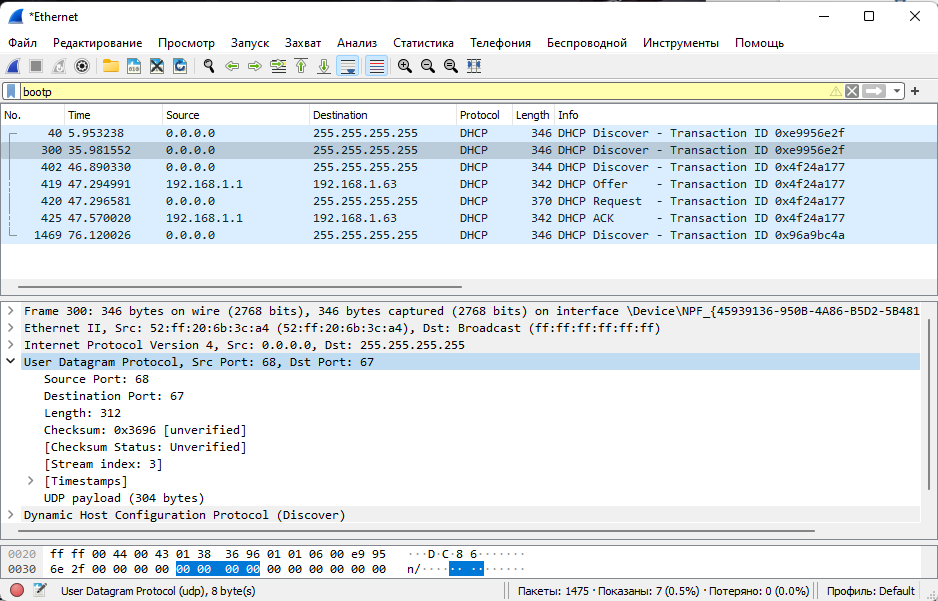
\includegraphics[width =\textwidth]{screenshots/1.png}}
\label{fig:image}
\end{center}
1) UDP

\begin{center}
\center{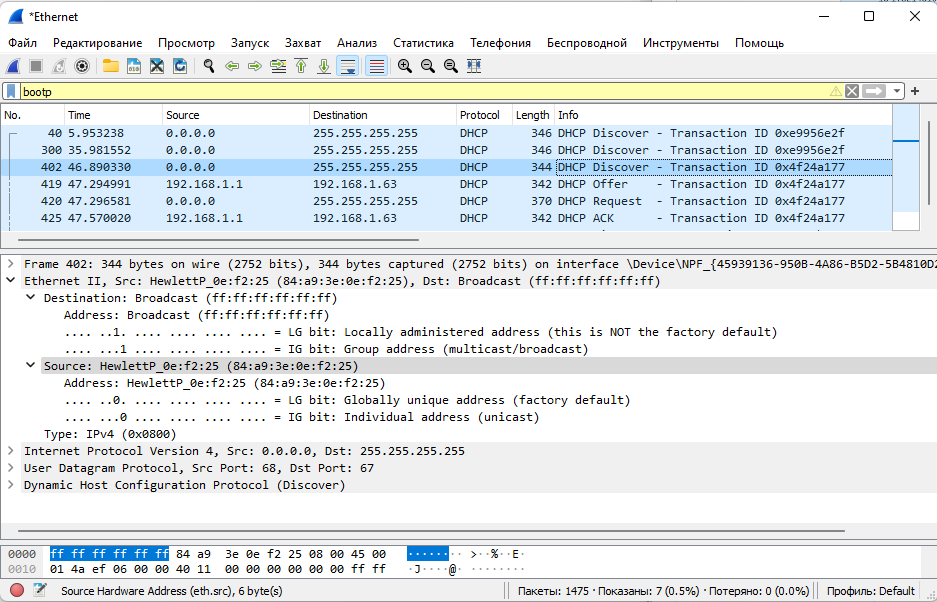
\includegraphics[width =\textwidth]{screenshots/2.png}}
\label{fig:image}
\end{center}
2) Address: HewlettP$\_$0e:f2:25 (84:a9:3e:0e:f2:25)

3) Request - Transaction ID 0x4f24a177

 ACK - Transaction ID 0x4f24a177
 
ID генерируется случайно клиентом, чтобы связать запрос с ответом на него

4) Src: 0.0.0.0, Dst: 255.255.255.255

5) 192.168.1.1

\begin{center}
\center{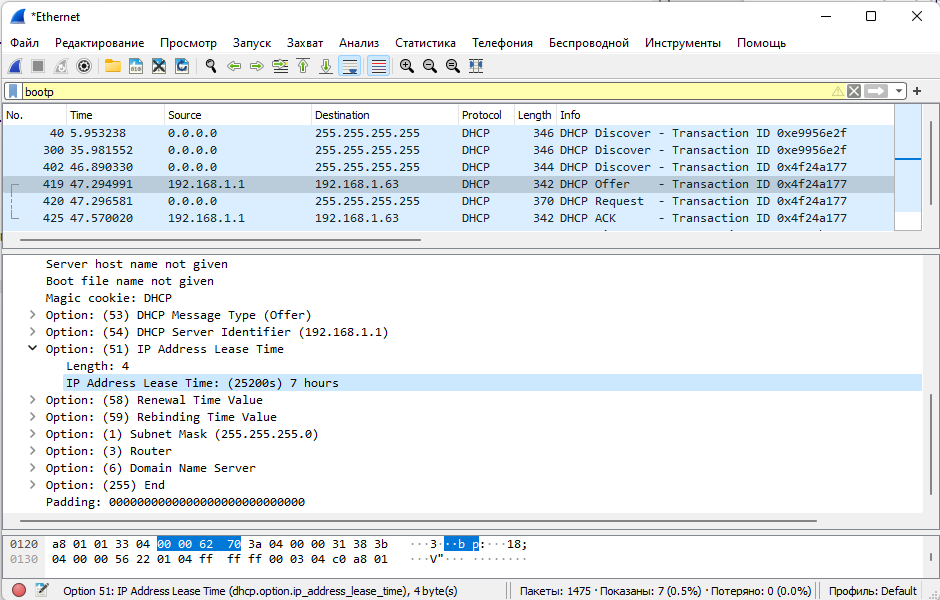
\includegraphics[width =\textwidth]{screenshots/3.png}}
\label{fig:image}
\end{center}
6) IP Address Lease Time: (25200s) 7 hours

Срок аренды показывает время, на которое адрес был выдан. Он ограничен, чтобы IP адреса занимали только активные клиенты
\end{document}








































